% The W tensor e1e1e2 + e1e2e1 + e2e1e1 drawn as a 2x2x2 cube of entries; front slice k=1, back slice k=2.
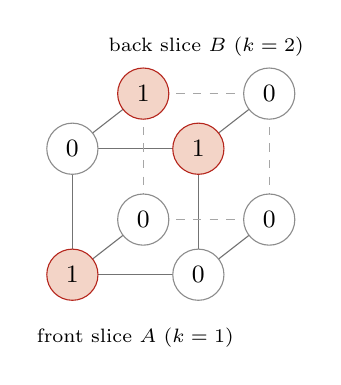
\begin{tikzpicture}[scale=1.0]
\draw[black!55] (0.00,0.00) -- (0.00,-1.60);
\draw[black!55] (0.00,0.00) -- (1.60,0.00);
\draw[black!55] (0.00,0.00) -- (0.90,0.70);
\draw[black!35,dashed] (0.90,0.70) -- (0.90,-0.90);
\draw[black!35,dashed] (0.90,0.70) -- (2.50,0.70);
\draw[black!55] (1.60,0.00) -- (1.60,-1.60);
\draw[black!55] (1.60,0.00) -- (2.50,0.70);
\draw[black!35,dashed] (2.50,0.70) -- (2.50,-0.90);
\draw[black!55] (0.00,-1.60) -- (1.60,-1.60);
\draw[black!55] (0.00,-1.60) -- (0.90,-0.90);
\draw[black!35,dashed] (0.90,-0.90) -- (2.50,-0.90);
\draw[black!55] (1.60,-1.60) -- (2.50,-0.90);
\node[circle,draw=BrickRed,fill=BrickRed!15,minimum size=6.5mm,inner sep=0pt,font=\small] at (0.90,0.70) {$1$};
\node[circle,draw=black!45,fill=white,minimum size=6.5mm,inner sep=0pt,font=\small] at (2.50,0.70) {$0$};
\node[circle,draw=black!45,fill=white,minimum size=6.5mm,inner sep=0pt,font=\small] at (0.90,-0.90) {$0$};
\node[circle,draw=black!45,fill=white,minimum size=6.5mm,inner sep=0pt,font=\small] at (2.50,-0.90) {$0$};
\node[circle,draw=black!45,fill=white,minimum size=6.5mm,inner sep=0pt,font=\small] at (0.00,0.00) {$0$};
\node[circle,draw=BrickRed,fill=BrickRed!15,minimum size=6.5mm,inner sep=0pt,font=\small] at (1.60,0.00) {$1$};
\node[circle,draw=BrickRed,fill=BrickRed!15,minimum size=6.5mm,inner sep=0pt,font=\small] at (0.00,-1.60) {$1$};
\node[circle,draw=black!45,fill=white,minimum size=6.5mm,inner sep=0pt,font=\small] at (1.60,-1.60) {$0$};
\node[font=\scriptsize,anchor=north] at (0.80,-2.15) {front slice $A$ ($k=1$)};
\node[font=\scriptsize,anchor=south] at (1.70,1.05) {back slice $B$ ($k=2$)};
\end{tikzpicture}
